%************************************************
\chapter{Risultati finali}
\label{cap:risultati}
%************************************************
\section{Introduzione}
Nel settore del parallel computing, i termini di successo di un progetto
sono le misure di performance. In questo lavoro di tesi � stata svolta
un'analisi attenta dei tempi e delle nostre misure di performance per poter
validare il lavoro. In particolare sono stati eseguiti differenti test su pi�
modelli.

Un primo test � stato il confronto della simulazione sequenziale con quella
parallela. Una volta accertata la loro stretta somiglianza, e in molti casi
l'esatta coincidenza dei valori, sono stati eseguiti ulteriori test riguardo
altre misure di performance e i tempi di esecuzione.

Questi ultimi test sono stati significativi poich� son serviti a validare il
lavoro di tesi. Si mostreranno nei paragrafi successivi alcuni grafici che
rappresentano i risultati dei test effettuati.

Di rilevale importanza � stata la scelta dei processori e delle schede video
utilizzate nell'esecuzione di questi test. Per quanto riguarda la simulazione
sequenziale sono stati utilizzati due processori Quad Xeon da 2.8 GHz con a
disposizione 4 core ciascuno. Questi due processori sono attualmente montati
sulla macchina \textit{Stromboli} situata al centro di calcolo ad alte
prestazioni (HPCC) dell'\textbf{Universit� della Calabria}. Per quanto riguarda
la simulazione parallela sono state utilizzate due schede grafiche diverse: una
GPU Nvidia Tesla K20c e una GPU Nvidia GeForce GT750M. La prima � situata, come
per la CPU Quad Xeon, al centro di calcolo ad alte prestazioni dell'Unical,
mentre la seconda � una delle pi� comuni schede video dei moderni laptop.

In forma tabellare � interessante mostrare le caratteristiche tecniche delle due
schede grafiche utilizzate:

\begin{table}[H]
\caption{Specifiche tecniche della GPU Nvidia Tesla K20c e della GPU Nvidia
GeForce GT750M.}
\label{tab:gpuk20c}
\centering
\begin{tabular}{p{0.35\textwidth}cc}
\toprule
\small Specifiche									&\small  Tesla K20c						&\small GeForce GT750M\\
\midrule

\small Nome della GPU								&\small  GK110							&\small GK107\\
\small Data di rilascio								&\small  12 Nov 2012					&\small 9 Gen 2013\\
\small GPU Clock									&\small  706 MHz						&\small 941 MHz\\
\small Memory clock									&\small  1300 MHz 5200 MHz eff.			&\small 1000
MHz 4000 MHz eff.\\
\small Numero di SM									&\small  2496							&\small 384
MHz\\
\small Numero di compute units						&\small  13								&\small 2\\
\small Floating point performance					&\small  3,524 GFLOPS					&\small 722.7
GFLOPS\\
\small Dimensione di memoria						&\small  5120 MB						&\small 2048 MB\\
\small Tipo di memoria								&\small  GDDR5							&\small GDDR5\\
\small Compute Capability							&\small  CUDA 3.5						&\small CUDA 3.0\\

\bottomrule
\end{tabular}
\end{table}

I test sono stati effettuati su diversi tipi di implementazioni di SCIARA-fv2.
L'insieme dei dati utilizzato tuttavia non � cambiato. In particolare sono stati
utilizzati i dati relativi all'attivit� svolta dal monte Etna nel 2006.
Si � utilizzata la libreria OpenCAL per implementare la versione sequenziale del
modello. In particolare � stata implementata anche una versione ottimizzata
tramite le celle attive.
Si � utilizzata invece, la libreria OpenCAL-CUDA per implementare la versione
parallela del modello, e, anche in questo caso � stata implementata una versione
ottimizzata tramite la tecnica delle celle attive.


\section{Confronto con i risultati}
Mostriamo ora i grafici relativi ai test effettuati sulle diverse
implementazioni. Confronteremo la versione sequenziale, implementata senza
l'ottimizzazione delle celle attive, con la versione parallela, implementata
anch'essa senza l'utilizzo di alcuna ottimizzazione.

\begin{figure}[H] \centering
\begin{tikzpicture}
\begin{axis} [xmin=0,xmax=10000,
ymin=0,ymax=1500,grid=major,title={Grafico dei
tempi},xlabel={Numero di step},ylabel={Tempo d'esecuzione (in secondi)},legend
style={anchor=north,at={(0.25,0.98)}}, width = 13cm,height = 7cm]

\addplot [thick,darkgray]
file {data/xeon_noopt.txt};
\addlegendentry{Quad Xeon da 2.8 GHz}

%\addplot [thick,cyan]
%file {data/K20_noopt.txt}; %% deve arrivare il file
%\addlegendentry{Tesla K20c}

\end{axis}
\end{tikzpicture}

\caption[Confronto tra SCIARA sequenziale e SCIARA parallelo senza
ottimizzazioni con l'utilizzo della configurazione con due crateri]{La versione
sequenziale � stata implementata con la libreria OpenCAL, quella parallela con OpenCAL-CUDA.}
\label{gr:noopt}
\end{figure}


Dal grafico si pu� notare come grazie all'architettura CUDA
e la GPGPU programming si possono incrementare le performance drasticamente.
Possiamo mostrare dunque, tramite il grafico \ref{gr:speedup_noopt}, l'andamento della
speedup (Vedi paragrafo \ref{par:misure_performance}) relativo al numero di
passi.

\begin{figure}[H] \centering
\begin{tikzpicture}
\begin{axis} [xmin=0,xmax=10000,
ymin=0,ymax=100,grid=major,title={Grafico della Speedup, senza
alcuna ottimizzazione},xlabel={Numero di step},ylabel={Speedup},legend
style={anchor=north,at={(0.25,0.98)}}, width = 13cm,height = 7cm]

\addplot [thick,orange]
file {data/speedup_noopt.txt};
\addlegendentry{Speedup}

\end{axis}

\end{tikzpicture}
\caption[Grafico della speedup, implementazione con l'ottimizzazione delle
celle attive e due crateri]{Il calcolo della speedup tra
implementazione sequenziale e parallela senza ottimizzazioni.}
\label{gr:speedup_noopt}
\end{figure}

Confrontiamo ora le due implementazioni, sequenziale e parallela, del
modello tramite l'ottimizzazione delle celle attive.

\begin{figure}[H] \centering
\begin{tikzpicture}
\begin{axis} [xmin=0,xmax=10000,
ymin=0,ymax=100,grid=major,title={Grafico dei tempi tramite
l'ottimizzazione delle celle attive},xlabel={Numero di step},ylabel={Tempo
d'esecuzione (in secondi)},legend style={anchor=north,at={(0.25,0.98)}}, width = 13cm,height = 7cm]

\addplot [thick,darkgray]
file {data/xeon_active.txt};
\addlegendentry{Quad Xeon da 2.8GHz}

\addplot [thick,cyan]
file {data/GT750M_active.txt};
\addlegendentry{NVIDIA GeForce GT750M}

\end{axis}

\end{tikzpicture}
\caption[Grafico dei tempi, confronto tra versione sequenziale e parallela
con ottimizzazione delle celle attive e configurazione con due crateri]{La versione sequenziale � stata implementata
con la libreria OpenCAL, quella parallela con OpenCAL-CUDA, entrambe le
versioni hanno utilizzato l'ottimizzazione delle celle attive.}
\label{gr:active_cells}
\end{figure}

Nel caso del grafico in fig. \ref{gr:active_cells} possiamo notare come la
versione sequenziale � pi� veloce rispetto a quella parallela dopo
un certo numero di step. Naturalmente la prima spiegazione plausibile � che le
due macchine a confronto non sono equiparabili a livello prestazionale. La Quad
Xeon � un processore ad alte prestazioni con un numero di operazioni al secondo
di gran lunga superiore ad una GPU come la GT 750M. Il secondo motivo � che
tramite l'ottimizzazione delle celle attive, per quanto riguarda il modello
SCIARA, vengono chiamate in causa per ogni step poche celle della nostra mappa.
Il loro numero ridotto non consente alle tecniche di parallelismo utilizzate di
mostrare la loro velocit� computazionale. 

Dato questo piccolo gap � stata implementata anche una seconda configurazione
per testare la libreria. Questa configurazione contiene un solo cambiamento
rispetto alla configurazione di base: la mappa dei crateri.
Nella nuova mappa dei crateri sono presenti 200 crateri diversi che a loro volta
genereranno un flusso pi� consistente di lava. In seguito mostreremo i grafici
dei test eseguiti con questa configurazione e si noter� come la GPGPU
programming tramite l'architettura CUDA ha apportato un grosso vantaggio in
termini di performance.

\begin{figure}[H] \centering
\begin{tikzpicture}
\begin{axis} [xmin=0,xmax=10000,
ymin=0,ymax=2500,grid=major,title={Grafico dei tempi tramite
l'ottimizzazione delle celle attive},xlabel={Numero di step},ylabel={Tempo
d'esecuzione (in secondi)},legend style={anchor=north,at={(0.25,0.98)}}, width = 13cm,height = 7cm]

\addplot [thick,darkgray]
file {data/xeon_active_200.txt};
\addlegendentry{Quad Xeon da 2.8GHz} 

\addplot [thick,cyan]
file {data/GT750M_active_200.txt};
\addlegendentry{NVIDIA GeForce GT750M}

\end{axis}

\end{tikzpicture}
\caption[Grafico dei tempi, confronto tra versione sequenziale e parallela
con ottimizzazione delle celle attive e configurazione con duecento crateri]{La
versione sequenziale � stata implementata con la libreria OpenCAL, quella parallela con OpenCAL-CUDA, entrambe le versioni hanno utilizzato l'ottimizzazione delle celle attive. In questo caso
sono stati utilizzati 200 crateri nella configurazione iniziale.}
\label{gr:active_cells_200}
\end{figure}

Vediamo insieme ora la speedup relativa all'implementazione con una
configurazione di 200 crateri.

\begin{figure}[H] \centering
\begin{tikzpicture}
\begin{axis} [xmin=0,xmax=10000,
ymin=0,ymax=50,grid=major,title={Grafico della Speedup con
l'ottimizzazione delle celle attive e con 200 crateri},xlabel={Numero di
step},ylabel={Speedup},legend style={anchor=north,at={(0.25,0.98)}}, width = 13cm,height = 7cm]

\addplot [thick,orange]
file {data/speedup_activecells_200.txt};
\addlegendentry{Speedup}

\end{axis}

\end{tikzpicture}
\caption[Grafico della speedup, implementazione con l'ottimizzazione delle
celle attive e duecento crateri]{Il calcolo della speedup tra implementazione
sequenziale e parallela con l'ottimizzazione delle celle attive e una configurazione contenente 200 crateri.}
\label{gr:speedup_active_200}
\end{figure}

\section{Risultati grafici}
\label{par:graphics_result}

Come accennato nel paragrafo precedente, un primo test � stato il confronto
della simulazione sequenziale con quella parallela. La libreria OpenCAL, cos�
come OpenCAL-CUDA, offrono delle funzionalit� per salvare l'output su file. Cos�
� stato fatto anche per il modello SCIARA. In particolare si � utilizzato il
software \textbf{Qgis} per la rappresentazione grafica dell'output.

Nelle seguenti figure, si mostrer� una rappresentazione della simulazione di
SCIARA dopo 10000 passi sia con due crateri che con 200 crateri.

\begin{figure}[H] 
\centering 
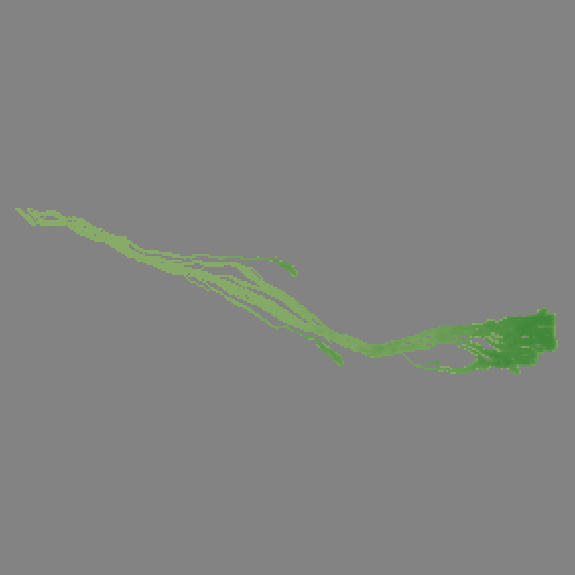
\includegraphics[width=0.5\columnwidth]{Immagini/2vent_thikness_} 
\caption[Simulazione con due crateri]{Simulazione mostrata dal software Qgis
con 2 crateri}
\label{fig:2vents} 
\end{figure}

\begin{figure}[H] 
\centering 
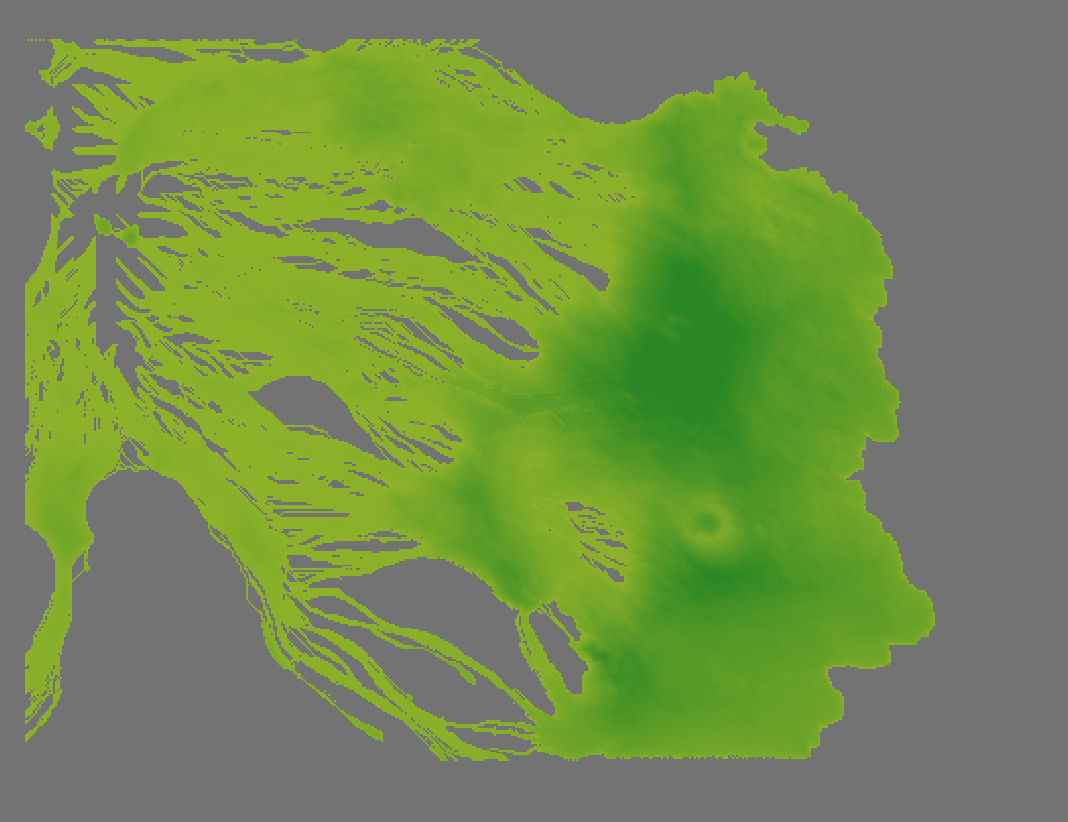
\includegraphics[width=0.5\columnwidth]{Immagini/200vent_thikness} 
\caption[Simulazione con duecento crateri]{Simulazione mostrata dal software
Qgis con 200 crateri}
\label{fig:200vent} 
\end{figure}
